\chapter{Polynomial Multiplication \& Fast Fourier Transform}

We shall investigate how to multiply two polynomial in a fast way step by step in this chapter to see how \textbf{FFT} works. In particular, it use a bit more space as it stores complex number, but makes a huge leap in terms of time complexity. FFT basically relys on \textbf{Divide and Conquer paradigm}, which is a method of solving problems that have non-overlapping subproblems. It does this by breaking up the main problem into multiple subproblems, and through solving these subproblems eventually solve the main problem. We shall see it step by step. Main goal of this chapter is to see that we can actually multiply two polynomial in \( O(n\log n) \), which is way way faster than the intuitive \( O(n^2) \).

\section{Problem Definition}

\begin{question}
	Let \( A, B, C \in \CC[X] \).
	\begin{itemize}
		\item \textbf{Input}: \( \{a_0, \ldots, a_{n-1}\}, \; \{b_0, \ldots, b_{n-1}\} \)
		      \begin{itemize}
			      \item assume \( n \) is the power of \( 2 \).
			      \item such represents the coefficients of the polynomial:
			            \[
				            A(x)= \sum_{i=0}^{n-1}a_i x^i \quad B(x) = \sum_{i=0}^{n-1}b_i x^i
			            \]
		      \end{itemize}
		\item \textbf{Output}: compute:
		      \[
			      C(x) = A(x)B(x) = \sum_{i=0}^{\mathbf{2n-2}}c_i x^i
		      \]

		      such problem of computing \( \{c_i\}_{i=0}^{2n-2} \) is called \underline{convolution}. Observe that:
		      \[
			      c_i = \sum_{0\leq j \leq i} a_j b_{i-j}
		      \]
	\end{itemize}
\end{question}

We note that for basic computing:
\begin{itemize}
	\item add: $C(x) = A(x) + B(x)$.
	\item substract: \( C(x) = A(x) - B(x) \).
	\item shift: \( C(x) = A(x) \cdot x^{10} \).
	\item Each of them takes \( O(n) \) operations.
\end{itemize}

See that the trivial algorithm that multiply the polynomial just like multiply the integers are just \( O(n^2) \).

\section{Divide and Conquer Algorithm}

One can rewrite \( A \) and \( B \) in the following sense:
\[
	\begin{aligned}
		A & = A_{hi}\cdot x^{\frac{n}{2}} + A_{lo} \\
		B & = B_{hi}\cdot x^{\frac{n}{2}} + B_{lo}
	\end{aligned}
\]

\begin{eg}
	\leavevmode
	\[
		A = 10x^5 - 9x^4 -x^3 +2x^2 +5x+9
	\]

	then:
	\( A_{hi} = 10 x^2 - 9x -1 \) and \( A_{lo} = 2x^2 +5x + 9 \) and \( A = A_{hi}\cdot x^3 + A_{lo} \).
\end{eg}

See that \( A_{hi}, A_{lo}, B_{hi}, B_{lo} \) are smaller polynomial, in the sense that they all have degree \( \frac{n}{2} - 1 \) but \( A,B \) have degree \( n-1 \).

Then observe that:
\[
	A\cdot B = A_{hi}B_{hi}x^n + (A_{hi}B_{lo} + A_{lo}B_{hi})x^{\frac{n}{2}} + A_{lo}B_{lo}
\]

thus, \textbf{one multiplication of degree-n polynomials} can be done using:
\begin{itemize}
	\item \textbf{4} multiplication of degree-\( \frac{n}{2} \) polynomials.
	\item \( O(1) \) additions/shifts of \( O(n) \) numbers.
\end{itemize}

The \textbf{recurrence relation} is given by:
\[
	\begin{aligned}
		T(n) & = 4T(\frac{n}{2}) + O(n) \\
		T(1) & = O(1)
	\end{aligned}
\]

By \textbf{Master Theorem} \ref{lem:master-sim}:
\[
	T(n) = O(n^2)
\]

\begin{note}
	As a side note, solving those kinds of recurrence relations can either be:
	\begin{itemize}
		\item Draw recursion tree, and calculate: if the overhead of each level is changing, then the recurrence relation is dominated by the level with the largest overhead; if the overhead of each level is same, then the recurrence relation is \( O(\text{number of levels} \times \text{overhead of each level}) \).
		\item Use master theorem and calculate by hand.
		\item Use \textbf{Induction}, basically \textbf{Guess and Check}.
	\end{itemize}
\end{note}

\section{Karatsuba's Algorithm}

Recall that:
\[
	A\cdot B = \mathcolor{blue}{A_{hi}B_{hi}x^n} + \mathcolor{red}{(A_{hi}B_{lo} + A_{lo}B_{hi})}x^{\frac{n}{2}} + \mathcolor{blue}{A_{lo}B_{lo}}
\]

One can actually deduce the red term from the blue term and reduce the times of calculating the multiplication by 1:
\[
	\mathcolor{red}{(A_{hi}B_{lo} + A_{lo}B_{hi})} = \mathcolor{blue}{A_{hi}B_{hi}x^n} + \mathcolor{blue}{A_{lo}B_{lo}} - (A_{hi} - A_{lo})(B_{hi} - B_{lo})
\]

New algorithm shall folow the steps:
\begin{enumerate}
	\item Compute \( T_{hi} = A_{hi}B_{hi} \) and \( T_{lo} = A_{lo}B_{lo} \) like before.
	\item Now compute \( S = (A_{hi} - A_{lo})(B_{hi} - B_{lo}) \).
	\item compute:
	      \[
		      A\cdot B = T_{hi}x^n + (T_{hi}+T_{lo} - S)x^{\frac{n}{2}} + T_{lo}
	      \]
\end{enumerate}

Thus we reduce the multiplication from \( 4 \) to \textbf{3}! The recurrence relation turns out to be:
\[
	\begin{aligned}
		T(n) & = 3T(\frac{n}{2}) + O(n) \\
		T(1) & = O(1)
	\end{aligned}
\]

thus by \textbf{Master Theorem} \ref{lem:master}:
\[
	T(n) = O(n^{\log_2 3})
\]

One may ask: \textbf{Can we reduce the number of subproblems to 2 instead?} If so we shall have:
\[
	\begin{aligned}
		T(n)          & = 2T(\frac{n}{2}) + O(n) \\
		T(1)          & = O(1)                   \\
		\implies T(n) & = O(n\log n)
	\end{aligned}
\]

which is exactly the FFT.

\section{Fast Fourier Transfrom}

\begin{definition}[\textbf{Representation of Polynomials}]
	Given \( A \in \CC[X] \), one can represent it in two ways:
	\begin{enumerate}
		\item Coefficients: \( \sum_{i=0}^{n-1}a_ix^i \).
		\item Point-value: \( \{(p_i, A(p_i))\}_{i=0}^{n-1} \).
	\end{enumerate}

	where the second one is from the \textbf{Linear Algebra Insight} \ref{lem:interpolation}.
\end{definition}

The key point here is: \textbf{It is easier to multiply polynomials in the point-value representation}. What shall be the results?
\begin{itemize}
	\item Given \( \{(p_i, A(p_i))\}_{i=0}^{2n-1} \) and \( \{(p_i, B(p_i))\}_{i=0}^{2n-1} \), note that we need \( 2n-1 \) points for each in order to \textbf{determine} \( C(x) \) later.
	\item Point-value representation of \( C \) is exactly:
	      \[
		      \{(p_i, A(p_i)B(p_i))\}_{i=0}^{2n-1}
	      \]
	      \begin{itemize}
		      \item It takes \( O(n) \) to \textbf{multiplications}.
		      \item This determines \( C \) because \( C \) has degree at most \( 2n-2 \).
	      \end{itemize}
\end{itemize}

But usually people store polynomials by its coefficients representation, as it is easier to evaluate the polynomial at any point in this case, thus we need coversion from coefficients representation to point-value representation and covert it back, and this conversion is where FFT is applied, and takes the most time complexity. See the following diagram.
\[
	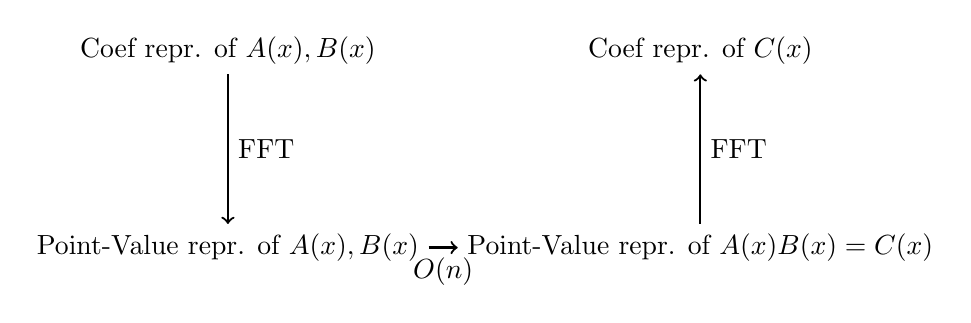
\begin{tikzpicture}[node distance=2cm, auto]
		\node (coefAB) {Coef repr. of $A(x), B(x)$};
		\node (pointAB) [below of=coefAB, node distance=2.5cm] {Point-Value repr. of $A(x), B(x)$};
		\node (pointC) [right of=pointAB, node distance=6cm] {Point-Value repr. of $A(x)B(x) = C(x)$};
		\node (coefC) [above of=pointC, node distance=2.5cm] {Coef repr. of $C(x)$};

		\draw[->, thick] (coefAB) -- (pointAB) node[midway, right] {FFT};
		\draw[->, thick] (pointAB) -- (pointC) node[midway, below] {$O(n)$};
		\draw[->, thick] (pointC) -- (coefC) node[midway, right] {FFT};
	\end{tikzpicture}
\]

One need to design a \textbf{special point set} \( \{p_0, \ldots, p_{2n-1}\} \), s.t.
\begin{enumerate}
	\item we can evaluate \( \{A(p_i), B(p_i)\}_{i=0}^{2n-1} \) at all points \( p_i \) in time \( O(n\log n) \).
	\item given \( \{C(p_i) = A(p_i) \cdot B(p_i)\}_{i=0}^{2n-1} \), we can compute the coefficients of \( C(x) \) in \( O(n\log n) \) time.
\end{enumerate}
